\documentclass{standalone}
\usepackage{tikz}
\usetikzlibrary{angles, arrows.meta}

\begin{document}

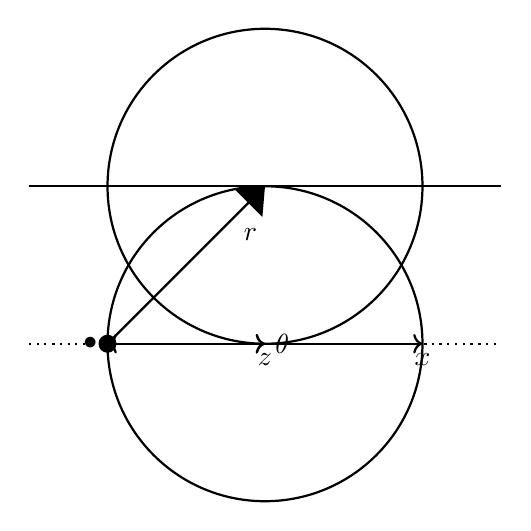
\begin{tikzpicture}[thick, scale=2]
    % Draw the outer circle representing the unperturbed bath free surface
    \draw (0,0) circle (1);
    
    % Draw the inner circle representing the unperturbed drop's free surface
    \draw (0,-1) circle (1);
    
    % Draw the droplet
    \filldraw[black] (-1, -1) circle (0.05) node[left] {$\bullet$};
    
    % Draw the radius vector
    \draw[-{Triangle[length=3mm, width=5mm]}] (-1, -1) -- (0, 0) 
        node[below right, pos=0.8] {$r$};
    
    % Draw the angle theta
    \coordinate (O) at (-1, -1);
    \coordinate (A) at (0, 0);
    \fill (O) circle (0.7pt); % Center of the droplet
    \draw[<->] (O) -- ++(0:1cm) node[right] {$\theta$}; % Polar angle theta
    
    % Draw the z-axis
    \draw[->] (-1, -1) -- (0, -1) node[below] {$z$};
    
    % Draw the x-axis
    \draw[->] (-1, -1) -- (1, -1) node[below] {$x$};
    
    % Draw the wavy line representing the unperturbed bath free surface
    \draw[solid] (-1.5, 0) sin (0, 0) cos (1.5, 0);
    
    % Draw the wavy line representing the perturbed bath free surface
    \draw[dotted] (-1.5, -1) sin (0, -1) cos (1.5, -1);

\end{tikzpicture}

\end{document}